\documentclass{article}
\usepackage{booktabs}
\usepackage[table]{xcolor}
\usepackage{makecell}
\usepackage{float}
\usepackage{graphicx}

\begin{document}
\title{NLSY97 Project}
\author{Rashad Dixon}
\date{\today}
\maketitle
\section{Analysis}
	Preliminary analysis of the distribution of arrests in 2002 shows a few commonalities across race.
Women of all identified races tend to be arrested at common rates. Black men are arrested more tha
n anyother race gender combination, more than double that of any other group. Additionally, men of 
all sampled races are arrested more frequently than their female counterparts when comparing within 
race. Mixed race (non-hispanic) show 0 mean arrests, though this is likely due to a lack of representation
 in the sample, or other sampling biases. 

\begin{figure}[H]
\centering
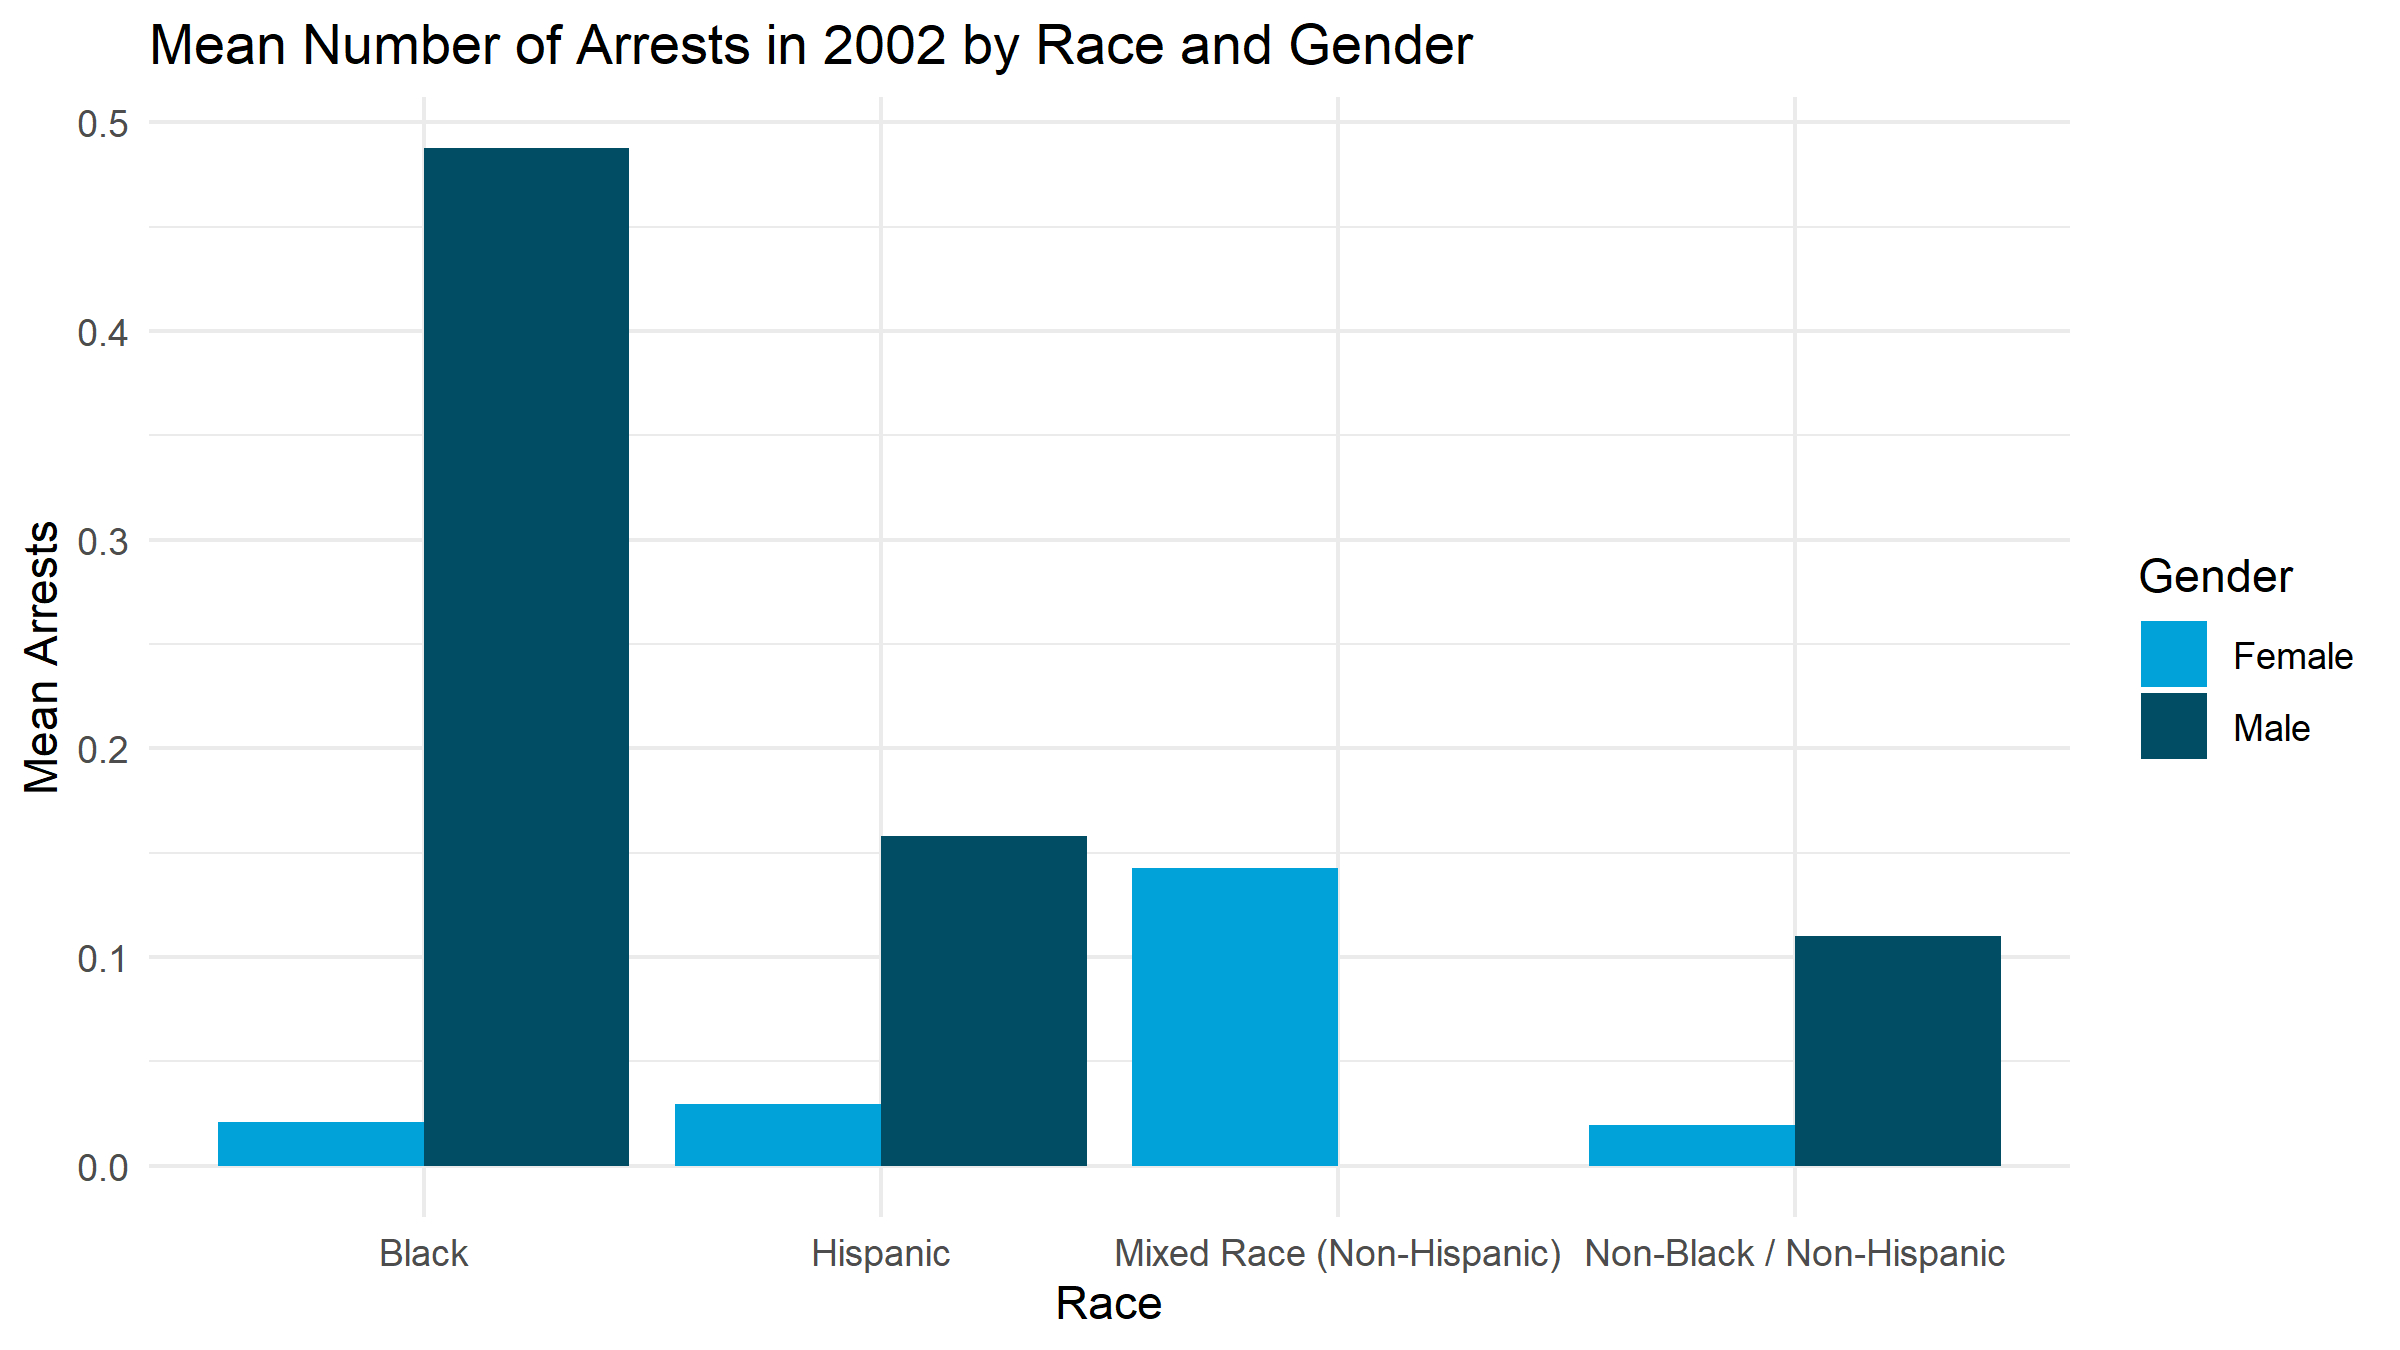
\includegraphics[scale = .75]{arrests_by_racegender.png}
\end{figure}

\begin{table}[H]

\caption{\label{tab:tab:summarystats}Mean arrests in 2002 by Race and Gender}
\centering
\begin{tabular}[t]{lrrrr}
\toprule
Gender & Black & Hispanic & Mixed Race Non Hispanic & Non Black Non Hispanic\\
\midrule
\cellcolor{gray!6}{Female} & \cellcolor{gray!6}{0.0211268} & \cellcolor{gray!6}{0.0298013} & \cellcolor{gray!6}{0.1428571} & \cellcolor{gray!6}{0.0193192}\\
Male & 0.4876712 & 0.1579509 & 0.0000000 & 0.1099476\\
\bottomrule
\end{tabular}
\end{table}

\section{Regression}
	The regression of Total 2002 arrests on the categorical variables race and gender provides us with coefficients
that relate demographics and arrests. The coefficients Non-Black/Non-Hispanic, Hispanic, and Male are significant at the .01 level. 
The regression provides a very low R\textsuperscript{2} of .015 which is likely due to the omission of significant variables like race, neighborhood, etc. 

% Table created by stargazer v.5.2.2 by Marek Hlavac, Harvard University. E-mail: hlavac at fas.harvard.edu
% Date and time: Sun, Jan 30, 2022 - 5:48:44 PM
\begin{table}[!htbp] \centering 
  \caption{Regression Output. Omitted category is Black Females.} 
  \label{tab:regression} 
\begin{tabular}{@{\extracolsep{5pt}}lc} 
\\[-1.8ex]\hline 
\hline \\[-1.8ex] 
 & \multicolumn{1}{c}{\textit{Dependent variable:}} \\ 
\cline{2-2} 
\\[-1.8ex] & Arrests in 2002 \\ 
\hline \\[-1.8ex] 
 Hispanic & $-$0.159$^{***}$ \\ 
  & (0.038) \\ 
  & \\ 
 Mixed Race (Non-Hispanic) & $-$0.174$^{**}$ \\ 
  & (0.083) \\ 
  & \\ 
 Non-Black / Non-Hispanic & $-$0.189$^{***}$ \\ 
  & (0.035) \\ 
  & \\ 
 Male & 0.194$^{***}$ \\ 
  & (0.022) \\ 
  & \\ 
 Constant & 0.155$^{***}$ \\ 
  & (0.026) \\ 
  & \\ 
\hline \\[-1.8ex] 
Observations & 8,621 \\ 
R$^{2}$ & 0.015 \\ 
Adjusted R$^{2}$ & 0.014 \\ 
Residual Std. Error & 1.019 (df = 8616) \\ 
F Statistic & 32.033$^{***}$ (df = 4; 8616) \\ 
\hline 
\hline \\[-1.8ex] 
\textit{Note:}  & \multicolumn{1}{r}{$^{*}$p$<$0.1; $^{**}$p$<$0.05; $^{***}$p$<$0.01} \\ 
\end{tabular} 
\end{table} 

\end{document}
